\section{Vibrational spectra from MD simulations}
\label{sec:vibrational_spectra_from_AIMD}

The simplest way to model the vibrational spectrum of the system is to perform a~vibrational analysis based on the eigenvalues of the Hessian matrix (the matrix of second derivatives of the potential energy). However, this analysis is valid at the fixed geometry of the system (at stationary points of the potential energy surface) and can include solvent effects only by the implicit models like PCM or through explicit including of the presence of some of the solvent molecules. Thus, for the case of liquid systems, to properly include effects of changing coordination, different conformations or appearance of hydrogen bonding and long distance effects, MD simulations need to be performed~\cite{aimd-spectra-review}. The vibrational spectrum can be obtained from a~MD trajectory by calculation of the appropriate autocorrelation function (AF): AF of the velocities for the power spectrum, AF of the dipole moment for the IR spectrum, and AF of the polarizability for the Raman spectrum~\cite{aimd-kirchner}. To gain results of a~desirable accuracy, the AIMD approach is preferable, because of problems with classical FFs to reproduce vibrational frequencies, especially in the case when HBs play a~significant role.

\begin{figure}[ht]
    \centering
    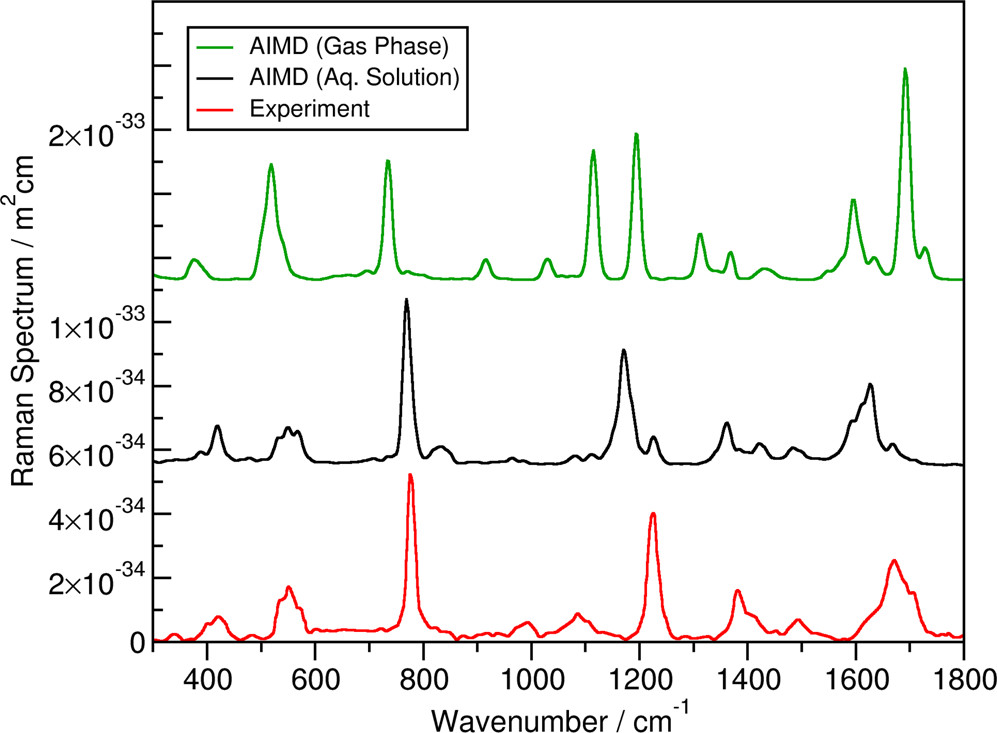
\includegraphics[width=0.65\textwidth]{img/1-introduction/raman-example.png}
    \caption{Raman spectrum of uracil calculated from AIMD simulation in gas phase and in aqueous solution~\cite{aimd-spectrum-5} compared with experimental spectrum~\cite{aimd-spectrum-8}}
    \label{fig:introduction-raman-example}
\end{figure}

AIMD was used successfully in the reproduction of experimental IR spectra. One example are systems with ILs consisting of EMIM cations and cyanamide-based anions~\cite{aimd-spectrum-1}. This approach was able to correctly show the existence of Fermi resonance on the spectrum of dicyanamide. For a~different system of droplets of EMIM acetate hydrogen bonding dynamics was investigated and the calculated power spectra were in good agreement with the experimental data~\cite{aimd-spectrum-2}.  Similar results were obtained for a~series of ILs based on cholinium~\cite{aimd-spectrum-3}. Other examples of the usage of the AIMD in prediction of vibrational spectra include studies on the IR spectra of iron(\textsc{ii}) polypyridyl complexes~\cite{aimd-spectrum-4}, resonance Raman spectra of uracil solution in water (with the use of time dependent DFT)~\cite{aimd-spectrum-5} and the C-H region in IR and Raman spectrum of dimethyl sulfoxide~\cite{aimd-spectrum-6}. Example of a~spectrum calculated from AIMD is presented in Figure~\ref{fig:introduction-raman-example}. One of recent articles mentions studies of spectral changes caused by interaction between lithium salt and solvent in EMIM-BF$_4$ and PC~\cite{aimd-spectrum-7}.

Usually, Born-Oppenheimer MD with DFT methods for obtaining wavefunctions for every time step of the simulation are used. Other approaches were also successful in this field. Car-Parinello MD (CPMD)~\cite{cpmd} was used for calculation of spectra of imidazolium based IL mixture with CO$_2$~\cite{cpmd-spectrum-1} as well as for Raman spectra of the cluster of ethyl ammonium nitrate~\cite{il-md-4}. A~semi-empirical method, DFTB, was used in analysis of the HBs in ethylammonium nitrate by studying theoretical IR spectra~\cite{dftb-spectrum-1} or for sodium salts in water~\cite{dftb-spectrum-2}.